\section{参数选择}
\subsection{弹簧管}
\begin{tabular}{@{}>{\raggedright\arraybackslash}p{0.4\linewidth}>{\centering\arraybackslash}p{0.4\linewidth}@{}}
    毛坯外径 & $\phi = 15mm$ \\
    毛坯中径 & $R = 50mm$ \\
    壁厚 & $h = 0.3mm$ \\
    轴比 & $\frac{a}{b} = 4$ \\
    中心角 & $\gamma'' = 250°$ \\
    材料 & 锡青铜(QSn4-0.3) \\
    泊松比 & $\mu = 0.3$ \\
    弹性模量E & $1.127 \times 10^5MPa$
\end{tabular}
\newline

如\autoref{FIGURE3.1}所示:
\begin{figure}[!htbp]
    \centering
    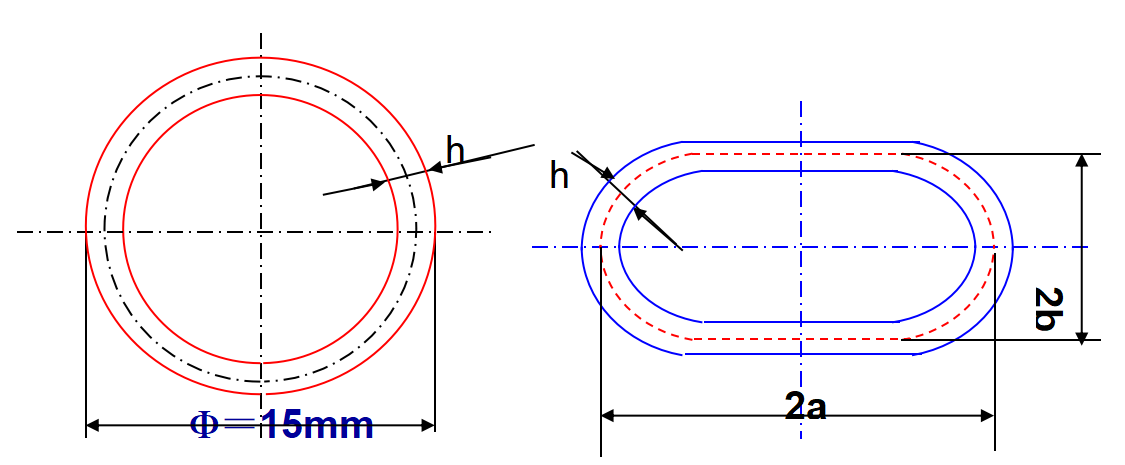
\includegraphics[width =\textwidth]{figures/3.1.png}
    \caption{弹簧管尺寸示意图}
    \label{FIGURE3.1}
\end{figure}
\subsection{曲柄滑块机构}
\begin{tabular}{@{}>{\raggedright\arraybackslash}p{0.4\linewidth}>{\raggedright\arraybackslash}p{0.4\linewidth}@{}}
相对杆长 : $\lambda=4$ &相对轴偏量 : $\varepsilon=1$\\
转动范围角 : $\alpha_p=18^\circ$ &初始位置角:$\alpha_0=-9^\circ$\\
终止位置角 : $\alpha_k=9^\circ$ &
\end{tabular}
\subsection{齿轮传动参数的选择}
\begin{tabular}{@{}>{\raggedright\arraybackslash}p{0.4\linewidth}>{\raggedright\arraybackslash}p{0.4\linewidth}@{}}
模数 : $m=0.25$ &小齿轮齿数 : $z_2=21$\\
传动比 : $i_{21}=15$& 
\end{tabular}
\subsection{标尺指针参数选择}
\begin{tabular}{@{}>{\raggedright\arraybackslash}p{0.4\linewidth}>{\raggedright\arraybackslash}p{0.4\linewidth}@{}}
分度尺寸:$3.375^{\circ}$ & 短标线长度:5mm\\
长标线长度:10mm & 指针与短标线重合长度:2mm\\
指针形状:楔杆形& 指针末端宽度:2mm
\end{tabular}
\subsection{游丝的选择}
\begin{tabular}{@{}>{\raggedright\arraybackslash}p{0.4\linewidth}>{\raggedright\arraybackslash}p{0.4\linewidth}@{}}
外径:$D_1=25mm$ & 内径:$D_2=5mm$\\
圈数:$n=10$ & 安装角度:$\phi_{min}=\frac{\pi}{2}$\\
宽度比:$\eta=6$ & 摩擦系数:$f=0.2$\\
当量摩擦系数:$f_v=0.314$ & 
\end{tabular}